% Generated by Sphinx.
\documentclass[a4paper,10pt,english]{manual}
\usepackage[utf8]{inputenc}
\usepackage[T1]{fontenc}
\usepackage{babel}
\usepackage{times}
\usepackage[Bjarne]{fncychap}
\usepackage{longtable}
\usepackage{sphinx}


\title{PyQwt Documentation}
\date{August 02, 2009}
\release{5.2.0}
\author{Gerard Vermeulen}
\newcommand{\sphinxlogo}{}
\renewcommand{\releasename}{Release}
\makeindex
\makemodindex
\newcommand\PYGZat{@}
\newcommand\PYGZlb{[}
\newcommand\PYGZrb{]}
\newcommand\PYGaz[1]{\textcolor[rgb]{0.00,0.63,0.00}{#1}}
\newcommand\PYGax[1]{\textcolor[rgb]{0.84,0.33,0.22}{\textbf{#1}}}
\newcommand\PYGay[1]{\textcolor[rgb]{0.00,0.44,0.13}{\textbf{#1}}}
\newcommand\PYGar[1]{\textcolor[rgb]{0.73,0.38,0.84}{#1}}
\newcommand\PYGas[1]{\textcolor[rgb]{0.25,0.44,0.63}{\textit{#1}}}
\newcommand\PYGap[1]{\textcolor[rgb]{0.00,0.44,0.13}{\textbf{#1}}}
\newcommand\PYGaq[1]{\textcolor[rgb]{0.38,0.68,0.84}{#1}}
\newcommand\PYGav[1]{\textcolor[rgb]{0.00,0.44,0.13}{\textbf{#1}}}
\newcommand\PYGaw[1]{\textcolor[rgb]{0.13,0.50,0.31}{#1}}
\newcommand\PYGat[1]{\textcolor[rgb]{0.73,0.38,0.84}{#1}}
\newcommand\PYGau[1]{\textcolor[rgb]{0.32,0.47,0.09}{#1}}
\newcommand\PYGaj[1]{\textcolor[rgb]{0.00,0.44,0.13}{#1}}
\newcommand\PYGak[1]{\textcolor[rgb]{0.14,0.33,0.53}{#1}}
\newcommand\PYGah[1]{\textcolor[rgb]{0.00,0.13,0.44}{\textbf{#1}}}
\newcommand\PYGai[1]{\textcolor[rgb]{0.73,0.38,0.84}{#1}}
\newcommand\PYGan[1]{\textcolor[rgb]{0.13,0.50,0.31}{#1}}
\newcommand\PYGao[1]{\textcolor[rgb]{0.25,0.44,0.63}{\textbf{#1}}}
\newcommand\PYGal[1]{\textcolor[rgb]{0.00,0.44,0.13}{\textbf{#1}}}
\newcommand\PYGam[1]{\textbf{#1}}
\newcommand\PYGab[1]{\textit{#1}}
\newcommand\PYGac[1]{\textcolor[rgb]{0.25,0.44,0.63}{#1}}
\newcommand\PYGaa[1]{\textcolor[rgb]{0.19,0.19,0.19}{#1}}
\newcommand\PYGaf[1]{\textcolor[rgb]{0.25,0.50,0.56}{\textit{#1}}}
\newcommand\PYGag[1]{\textcolor[rgb]{0.13,0.50,0.31}{#1}}
\newcommand\PYGad[1]{\textcolor[rgb]{0.00,0.25,0.82}{#1}}
\newcommand\PYGae[1]{\textcolor[rgb]{0.13,0.50,0.31}{#1}}
\newcommand\PYGaZ[1]{\textcolor[rgb]{0.25,0.44,0.63}{#1}}
\newcommand\PYGbf[1]{\textcolor[rgb]{0.00,0.44,0.13}{#1}}
\newcommand\PYGaX[1]{\textcolor[rgb]{0.25,0.44,0.63}{#1}}
\newcommand\PYGaY[1]{\textcolor[rgb]{0.00,0.44,0.13}{#1}}
\newcommand\PYGbc[1]{\textcolor[rgb]{0.78,0.36,0.04}{#1}}
\newcommand\PYGbb[1]{\textcolor[rgb]{0.00,0.00,0.50}{\textbf{#1}}}
\newcommand\PYGba[1]{\textcolor[rgb]{0.02,0.16,0.45}{\textbf{#1}}}
\newcommand\PYGaR[1]{\textcolor[rgb]{0.25,0.44,0.63}{#1}}
\newcommand\PYGaS[1]{\textcolor[rgb]{0.13,0.50,0.31}{#1}}
\newcommand\PYGaP[1]{\textcolor[rgb]{0.05,0.52,0.71}{\textbf{#1}}}
\newcommand\PYGaQ[1]{\textcolor[rgb]{0.78,0.36,0.04}{\textbf{#1}}}
\newcommand\PYGaV[1]{\textcolor[rgb]{0.25,0.50,0.56}{\textit{#1}}}
\newcommand\PYGaW[1]{\textcolor[rgb]{0.05,0.52,0.71}{\textbf{#1}}}
\newcommand\PYGaT[1]{\textcolor[rgb]{0.73,0.38,0.84}{#1}}
\newcommand\PYGaU[1]{\textcolor[rgb]{0.13,0.50,0.31}{#1}}
\newcommand\PYGaJ[1]{\textcolor[rgb]{0.56,0.13,0.00}{#1}}
\newcommand\PYGaK[1]{\textcolor[rgb]{0.25,0.44,0.63}{#1}}
\newcommand\PYGaH[1]{\textcolor[rgb]{0.50,0.00,0.50}{\textbf{#1}}}
\newcommand\PYGaI[1]{\fcolorbox[rgb]{1.00,0.00,0.00}{1,1,1}{#1}}
\newcommand\PYGaN[1]{\textcolor[rgb]{0.73,0.73,0.73}{#1}}
\newcommand\PYGaO[1]{\textcolor[rgb]{0.00,0.44,0.13}{#1}}
\newcommand\PYGaL[1]{\textcolor[rgb]{0.02,0.16,0.49}{#1}}
\newcommand\PYGaM[1]{\colorbox[rgb]{1.00,0.94,0.94}{\textcolor[rgb]{0.25,0.50,0.56}{#1}}}
\newcommand\PYGaB[1]{\textcolor[rgb]{0.25,0.44,0.63}{#1}}
\newcommand\PYGaC[1]{\textcolor[rgb]{0.33,0.33,0.33}{\textbf{#1}}}
\newcommand\PYGaA[1]{\textcolor[rgb]{0.00,0.44,0.13}{#1}}
\newcommand\PYGaF[1]{\textcolor[rgb]{0.63,0.00,0.00}{#1}}
\newcommand\PYGaG[1]{\textcolor[rgb]{1.00,0.00,0.00}{#1}}
\newcommand\PYGaD[1]{\textcolor[rgb]{0.00,0.44,0.13}{\textbf{#1}}}
\newcommand\PYGaE[1]{\textcolor[rgb]{0.25,0.50,0.56}{\textit{#1}}}
\newcommand\PYGbg[1]{\textcolor[rgb]{0.44,0.63,0.82}{\textit{#1}}}
\newcommand\PYGbe[1]{\textcolor[rgb]{0.40,0.40,0.40}{#1}}
\newcommand\PYGbd[1]{\textcolor[rgb]{0.25,0.44,0.63}{#1}}
\newcommand\PYGbh[1]{\textcolor[rgb]{0.00,0.44,0.13}{\textbf{#1}}}
\begin{document}

\maketitle
\tableofcontents



\resetcurrentobjects
\hypertarget{--doc-introduction}{}

\chapter{Introduction}

PyQwt is a set of Python bindings for the
\href{http://qwt.sourceforge.net}{Qwt}
library featuring fast plotting of Python lists and tuples and the
powerful multi-dimensional arrays provided by
\href{http://numpy.scipy.org}{NumPy}, the fundamental package for
efficient scientific and engineering computing in Python. \footnote{
The older numerical Python extension packages,
\href{http://www.stsci.edu/resources/software\_hardware/numarray}{numarray}
and
\href{http://numpy.scipy.org/}{Numeric}
are deprecated.
}


\section{NumPy}

The \href{http://numpy.scipy.org}{NumPy} package extends Python with
multi-dimensional arrays and a complete set of `standard' functions
and operators to manipulate the arrays. NumPy turns Python into is an
ideal language experimental numerical and scientific computing (as
powerful as APL, MatLab, IDL and others, but much more elegant).

If you do not have a mathematical background, you can think of a
1-dimensional array as a column in a spreadsheet.  The spreadsheet
lets you change whole columns element by element in one single
statement. In a similar way, NumPy lets you change whole arrays
element by element in one single statement as illustrated by the
following snippet:

\begin{Verbatim}[commandchars=@\[\]]
@PYGaQ[@textgreater[]@textgreater[]@textgreater[] ]@PYGal[import] @PYGaW[numpy] @PYGal[as] @PYGaW[np]
@PYGaQ[@textgreater[]@textgreater[]@textgreater[] ]x @PYGbe[=] np@PYGbe[.]arange(@PYGaw[0.0], @PYGaw[10.0], @PYGaw[3.0])
@PYGaQ[@textgreater[]@textgreater[]@textgreater[] ]y @PYGbe[=] np@PYGbe[.]sin(x)
@PYGaQ[@textgreater[]@textgreater[]@textgreater[] ]x
@PYGaa[array(@PYGZlb[] 0.,  3.,  6.,  9.@PYGZrb[])]
@PYGaQ[@textgreater[]@textgreater[]@textgreater[] ]y
@PYGaa[array(@PYGZlb[] 0.        ,  0.14112001, -0.2794155 ,  0.41211849@PYGZrb[])]
@PYGaQ[@textgreater[]@textgreater[]@textgreater[] ]x@PYGbe[*]x
@PYGaa[array(@PYGZlb[]  0.,   9.,  36.,  81.@PYGZrb[])]
\end{Verbatim}

The statement:

\begin{Verbatim}[commandchars=@\[\]]
@PYGaQ[@textgreater[]@textgreater[]@textgreater[] ]np@PYGbe[.]arange(@PYGaw[0.0], @PYGaw[10.0], @PYGaw[3.0])
\end{Verbatim}

returns a NumPy array of 4 equidistant points from 0 to 9 inclusive:

\begin{Verbatim}[commandchars=@\[\]]
array(@PYGZlb[] @PYGaw[0.], @PYGaw[3.], @PYGaw[6.], @PYGaw[9.]@PYGZrb[])
\end{Verbatim}

The statements \code{y = np.sin(x)} and \code{x*x} show that NumPy
arrays are manipulated element by element.
All this in has been coded in C, for a manifold speedup with respect
to pure Python.

You can think of a 2-dimension array as a spreadsheet: in both cases
you you can operate on blocks, columns, rows, slices of colums, slices
of rows or individual elements.

Want to learn more?
Look at the
\href{http://www.scipy.org/Tentative\_NumPy\_Tutorial}{Tentative NumPy Tutorial}
for a tutorial or at the
\href{http://www.tramy.us/numpybook.pdf}{Guide to NumPy}
for an advanced book.


\section{Qwt}

\href{http://qwt.sourceforge.net}{Qwt} is a C++ library based on the
\href{http://trolltech.com/products/qt}{Qt GUI framework}.
The Qwt library contains widgets useful for writing technical,
scientific, and financial programs.
It includes the following widgets:
\begin{description}
\item[QwtCompass]
a very fancy QDial-like widget to display and control a direction.

\item[QwtCounter]
a QSpinBox-like widget to display and control a bounded floating
point value.

\item[QwtDial]
a QDial-like widget to display and control a floating point value.

\item[QwtKnob]
a potentiometer-like widget to display and control a bounded
floating point value.

\item[QwtPlot]
a widget to plot data in two dimensions.

\item[QwtSlider]
a QSlider-like widget to display and control a bounded floating
point value.

\item[QwtThermo]
a thermometer-like widget to display a floating point value.

\item[QwtWheel]
a wheel-like widget with its axis parallel to the computer screen
to control a floating point value over a very large range in very
small steps.

\end{description}

See the \href{http://qwt.sourceforge.net}{Qwt manual} for a complete
overview of the Qwt library.


\section{PyQwt with NumPy}

PyQwt is mostly used to write graphical user interface applications.
However, the following snippet shows how to use PyQwt in combination
with NumPy from the command line interpreter.
Line by line explanations follow the snippet:

\begin{Verbatim}[commandchars=@\[\]]
@PYGaQ[@textgreater[]@textgreater[]@textgreater[] ]@PYGal[import] @PYGaW[numpy] @PYGal[as] @PYGaW[np]
@PYGaQ[@textgreater[]@textgreater[]@textgreater[] ]@PYGal[from] @PYGaW[PyQt4.Qt] @PYGal[import] @PYGbe[*]
@PYGaQ[@textgreater[]@textgreater[]@textgreater[] ]@PYGal[from] @PYGaW[PyQt4.Qwt5] @PYGal[import] @PYGbe[*]
@PYGaQ[@textgreater[]@textgreater[]@textgreater[] ]@PYGal[from] @PYGaW[PyQt4.Qwt5.qplt] @PYGal[import] @PYGbe[*]
@PYGaQ[@textgreater[]@textgreater[]@textgreater[] ]application @PYGbe[=] QApplication(@PYGZlb[]@PYGZrb[])
@PYGaQ[@textgreater[]@textgreater[]@textgreater[] ]x @PYGbe[=] np@PYGbe[.]arange(@PYGbe[-]@PYGaw[2]@PYGbe[*]np@PYGbe[.]pi, @PYGaw[2]@PYGbe[*]np@PYGbe[.]pi, @PYGaw[0.01])
@PYGaQ[@textgreater[]@textgreater[]@textgreater[] ]p @PYGbe[=] Plot(
@PYGaQ[... ] Curve(x, np@PYGbe[.]cos(x), Pen(Magenta, @PYGaw[2]), @PYGaB["]@PYGaB[cos(x)]@PYGaB["]),
@PYGaQ[... ] Curve(x, np@PYGbe[.]exp(x), Pen(Red), @PYGaB["]@PYGaB[exp(x)]@PYGaB["], Y2),
@PYGaQ[... ] Axis(Y2, Log),
@PYGaQ[... ] @PYGaB["]@PYGaB[PyQwt using Qwt-]@PYGbg[@%s]@PYGaB[ -- http://qwt.sf.net]@PYGaB["] @PYGbe[@%] QWT@_VERSION@_STR)
@PYGaQ[@textgreater[]@textgreater[]@textgreater[] ]QPixmap@PYGbe[.]grabWidget(p)@PYGbe[.]save(@PYGaB[']@PYGaB[cli-plot-1.png]@PYGaB['], @PYGaB[']@PYGaB[PNG]@PYGaB['])
@PYGaa[True]
@PYGaQ[@textgreater[]@textgreater[]@textgreater[] ]x @PYGbe[=] x@PYGZlb[]@PYGaw[0]:@PYGbe[-]@PYGaw[1]:@PYGaw[10]@PYGZrb[]
@PYGaQ[@textgreater[]@textgreater[]@textgreater[] ]p@PYGbe[.]plot(
@PYGaQ[... ] Curve(x, np@PYGbe[.]cos(x@PYGbe[-]np@PYGbe[.]pi@PYGbe[/]@PYGaw[4]), Symbol(Circle, Yellow), @PYGaB["]@PYGaB[circle]@PYGaB["]),
@PYGaQ[... ] Curve(x, np@PYGbe[.]cos(x@PYGbe[+]np@PYGbe[.]pi@PYGbe[/]@PYGaw[4]), Pen(Blue), Symbol(Square, Cyan), @PYGaB["]@PYGaB[square]@PYGaB["]))
@PYGaQ[@textgreater[]@textgreater[]@textgreater[] ]QPixmap@PYGbe[.]grabWidget(p)@PYGbe[.]save(@PYGaB[']@PYGaB[cli-plot-2.png]@PYGaB['], @PYGaB[']@PYGaB[PNG]@PYGaB['])
@PYGaa[True]
\end{Verbatim}

The statements:

\begin{Verbatim}[commandchars=@\[\]]
@PYGaQ[@textgreater[]@textgreater[]@textgreater[] ]@PYGal[import] @PYGaW[numpy] @PYGal[as] @PYGaW[np]
@PYGaQ[@textgreater[]@textgreater[]@textgreater[] ]@PYGal[from] @PYGaW[PyQt4.Qt] @PYGal[import] @PYGbe[*]
@PYGaQ[@textgreater[]@textgreater[]@textgreater[] ]@PYGal[from] @PYGaW[PyQt4.Qwt5] @PYGal[import] @PYGbe[*]
@PYGaQ[@textgreater[]@textgreater[]@textgreater[] ]@PYGal[from] @PYGaW[PyQt4.Qwt5.qplt] @PYGal[import] @PYGbe[*]
\end{Verbatim}

import numpy, PyQt4, Qwt5 and qplt.
The statement:

\begin{Verbatim}[commandchars=@\[\]]
@PYGaQ[@textgreater[]@textgreater[]@textgreater[] ]application @PYGbe[=] QApplication(@PYGZlb[]@PYGZrb[])
\end{Verbatim}

initializes and starts the Qt library so that it handles mouse
movements, mouse button presses, and keyboard key presses. \footnote{
PyQt-4.3.x and later support displaying Qt widgets from the
Python command line interpreter.
}
The statement:

\begin{Verbatim}[commandchars=@\[\]]
@PYGaQ[@textgreater[]@textgreater[]@textgreater[] ]x @PYGbe[=] np@PYGbe[.]arange(@PYGbe[-]@PYGaw[2]@PYGbe[*]np@PYGbe[.]pi, @PYGaw[2]@PYGbe[*]np@PYGbe[.]pi, @PYGaw[0.01])
\end{Verbatim}

creates an array with elements increasing from -2*np.pi to 2*np.pi in
steps of 0.01.
The statement:

\begin{Verbatim}[commandchars=@\[\]]
@PYGaQ[@textgreater[]@textgreater[]@textgreater[] ]p @PYGbe[=] Plot(
@PYGaQ[... ] Curve(x, np@PYGbe[.]cos(x), Pen(Magenta, @PYGaw[2]), @PYGaB["]@PYGaB[cos(x)]@PYGaB["]),
@PYGaQ[... ] Curve(x, np@PYGbe[.]exp(x), Pen(Red), @PYGaB["]@PYGaB[exp(x)]@PYGaB["], Y2),
@PYGaQ[... ] Axis(Y2, Log),
@PYGaQ[... ] @PYGaB["]@PYGaB[PyQwt using Qwt-]@PYGbg[@%s]@PYGaB[ -- http://qwt.sf.net]@PYGaB["] @PYGbe[@%] QWT@_VERSION@_STR)
\end{Verbatim}

creates and shows a plot widget with two curves and an additional
right vertical logarithmic axis.
The statement:

\begin{Verbatim}[commandchars=@\[\]]
@PYGaQ[@textgreater[]@textgreater[]@textgreater[] ]QPixmap@PYGbe[.]grabWidget(p)@PYGbe[.]save(@PYGaB[']@PYGaB[cli-plot-1.png]@PYGaB['], @PYGaB[']@PYGaB[PNG]@PYGaB['])
@PYGaa[True]
\end{Verbatim}

takes a snapshot of the plot widget and saves it into a file:

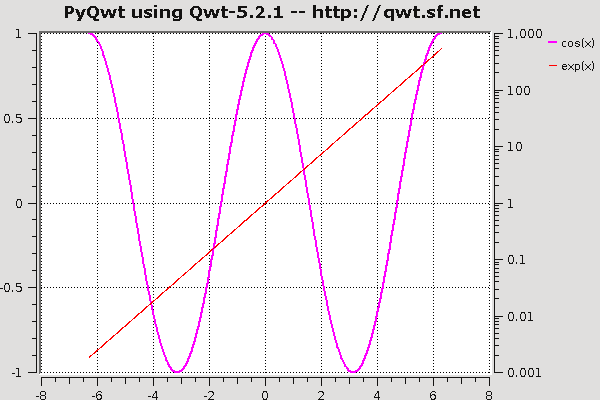
\includegraphics{cli-plot-1.png}

The statement:

\begin{Verbatim}[commandchars=@\[\]]
@PYGaQ[@textgreater[]@textgreater[]@textgreater[] ]x @PYGbe[=] x@PYGZlb[]@PYGaw[0]:@PYGbe[-]@PYGaw[1]:@PYGaw[10]@PYGZrb[]
\end{Verbatim}

creates a new array from the old one by selecting every tenth element
start from the index 0.
The statement:

\begin{Verbatim}[commandchars=@\[\]]
@PYGaQ[@textgreater[]@textgreater[]@textgreater[] ]p@PYGbe[.]plot(
@PYGaQ[... ] Curve(x, np@PYGbe[.]cos(x@PYGbe[-]np@PYGbe[.]pi@PYGbe[/]@PYGaw[4]), Symbol(Circle, Yellow), @PYGaB["]@PYGaB[circle]@PYGaB["]),
@PYGaQ[... ] Curve(x, np@PYGbe[.]cos(x@PYGbe[+]np@PYGbe[.]pi@PYGbe[/]@PYGaw[4]), Pen(Blue), Symbol(Square, Cyan),
@PYGaQ[... ] @PYGaB["]@PYGaB[square]@PYGaB["]))
\end{Verbatim}

plots two new curves on the widget using the new array.
The statement:

\begin{Verbatim}[commandchars=@\[\]]
@PYGaQ[@textgreater[]@textgreater[]@textgreater[] ]QPixmap@PYGbe[.]grabWidget(p)@PYGbe[.]save(@PYGaB[']@PYGaB[cli-plot-2.png]@PYGaB['], @PYGaB[']@PYGaB[PNG]@PYGaB['])
@PYGaa[True]
\end{Verbatim}

takes a snapshot of the plot widget and saves it into a file:

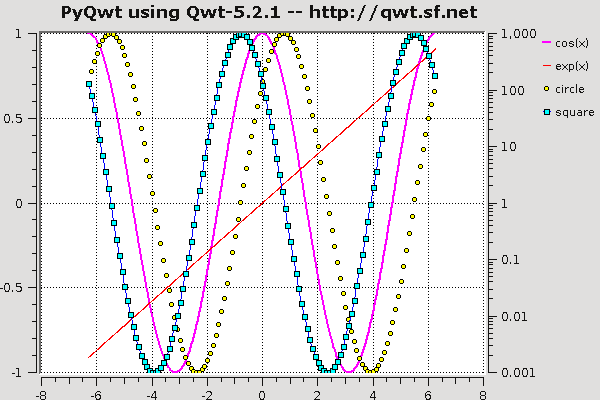
\includegraphics{cli-plot-2.png}
\hypertarget{getting-help}{}

\section{Getting help}

PyQwt and PyQwt3D have a low volume mailing list to answer questions
on installation problems and how to use the more advanced features.
In particular, many of the more advanced examples using object
oriented programming have been written to answer questions.
Most questions help to improve PyQwt!

Please,
\href{http://lists.sourceforge.net/lists/listinfo/pyqwt-users}{subscribe}
to the mailing list before posting on the
\href{mailto:pyqwt-users@lists.sourceforge.net}{mailing list}.

The mailing list is a subscribers only list and mail from
non-subscribers is deferred to filter spam (more than 95 \% of the mail
by non-subscribers is spam and mail by non-subscribers is rejected).

The mailing list is configured to garantee anonimity as much as
possible.

\resetcurrentobjects
\hypertarget{--doc-installation}{}

\chapter{Installation}


\section{Source Code Installation}


\subsection{Build Prerequisites}

Recommended build prerequisites for PyQwt-5.2.0 are:
\begin{enumerate}
\item {} 
\href{http://www.python.org}{Python}, version 2.6.x and 2.5.x are
supported.

\item {} 
\href{http://trolltech.com/products/qt}{Qt}, version 4.5.x, 4.4.x,
4.3.x, and 3.3.x  are supported.

\item {} 
\href{http://www.riverbankcomputing.co.uk/software/sip/intro}{SIP},
version 4.8.x and 4.7.x (x \textgreater{} 3) are supported.

\item {} 
\href{http://www.riverbankcomputing.co.uk/software/pyqt/intro}{PyQt}
for Mac OS X, Windows, and/or X11, version 4.5.x, 4.4.x, 4.3.x,
3.18.x, and 3.17.x are supported.

\item {} 
optionally \href{http://www.scipy.org/NumPy}{NumPy}, version 1.3.x,
1.2.x, and 1.1.x are supported.

\item {} 
optionally \href{http://qwt.sourceforge.net}{Qwt}, version 5.2.x,
5.1.x, and 5.0.x are supported.

\end{enumerate}

The source package
\href{http://prdownloads.sourceforge.net/pyqwt/PyQwt-5.2.0.tar.gz}{PyQwt-5.2.0.tar.gz}
contains a snapshot of the Qwt-5.2 subversion bug fix branch which may
fix some bugs in Qwt-5.2.0.
I recommend to compile and link the bug fix branch statically into PyQwt.

To exploit the full power of PyQwt, you should install at least one of
the numerical Python extensions:
\begin{itemize}
\item {} 
\href{http://www.scipy.org/NumPy}{NumPy}

\item {} 
\href{http://www.stsci.edu/resources/software\_hardware/numarray}{numarray}

\item {} 
\href{http://numpy.scipy.org/}{Numeric}

\end{itemize}

and built PyQwt with support for the numerical Python extension(s) of
your choice.  However, only NumPy is actively developed and numarray and
Numeric are deprecated.

PyQwt-5.2.0 and recent versions of the numerical Python extensions support
the \href{http://numpy.scipy.org/array\_interface.shtml}{N-D array interface}
protocol.  Therefore, PyQwt supports those extensions, even if they have not
been installed when PyQwt has been built. In this case, the functionality is
somewhat reduced, since conversion from an QImage to a Numerical
Python array is not supported.


\subsection{Installation}

The installation procedure consists of three steps:
\begin{enumerate}
\item {} 
Unpack PyQwt-5.2.0.tar.gz.

\item {} 
Invoke the following commands to build PyQwt-5.2.0 for Qt-4:

\begin{Verbatim}[commandchars=@\[\]]
cd PyQwt-5.2.0
cd configure
python configure.py -Q ../qwt-5.2
make
make install
\end{Verbatim}

or invoke the commands to build PyQwt-5.2.0 for Qt-3:

\begin{Verbatim}[commandchars=@\[\]]
cd PyQwt-5.2.0
cd configure
python configure.py -3 -Q ../qwt-5.2
make
make install
\end{Verbatim}

This assumes that the correct Python interpreter is on your path. Replace
\textbf{make} by \textbf{nmake}, if you use Microsoft Visual C++.
The commands build PyQwt against the included Qwt subversion snapshot and
install PyQwt.
Test the installation by playing with the example programs.

\item {} 
Fine tune (optional):
\begin{itemize}
\item {} 
to use a Qwt library already installed on your system invoke
commands similar to:

\begin{Verbatim}[commandchars=@\[\]]
python configure.py -I/usr/include/qwt -lqwt
make
make install
\end{Verbatim}

where the Qwt header files are assumed to be installed in
\code{/usr/include/qwt}.

If the linker fails to find the qwt library, add:

\begin{Verbatim}[commandchars=@\[\]]
-L /directory/with/qwt/library
\end{Verbatim}

to the \textbf{configure.py} options.

\end{itemize}

The configure.py script takes many options. The command:

\begin{Verbatim}[commandchars=@\[\]]
python configure.py -h
\end{Verbatim}

displays a full list of the available options

\begin{Verbatim}[commandchars=@\[\]]
Usage: python configure.py @PYGZlb[]options@PYGZrb[]

Each option takes at most one argument, but some options
accumulate arguments when repeated. For example, invoke:

	python configure.py -I . -I ..

to search the current *and* parent directories for headers.

Options:
  -h, --help            show this help message and exit

  Common options:
    -3, --qt3           build for Qt3 and PyQt @PYGZlb[]default Qt4@PYGZrb[]
    -4, --qt4           build for Qt4 and PyQt4 @PYGZlb[]default Qt4@PYGZrb[]
    -Q /sources/of/qwt, --qwt-sources=/sources/of/qwt
                        compile and link the Qwt source files in
                        /sources/of/qwt statically into PyQwt
    -I /usr/lib/qt3/include/qwt, --extra-include-dirs=/usr/lib/qt3/include/qwt
                        add an extra directory to search for headers (the
                        compiler must be able to find the Qwt headers without
                        the -Q option)
    -L /usr/lib/qt3/lib, --extra-lib-dirs=/usr/lib/qt3/lib
                        add an extra directory to search for libraries (the
                        linker must be able to find the Qwt library without
                        the -Q option)
    -j N, --jobs=N      concatenate the SIP generated code into N files
                        @PYGZlb[]default 1 per class@PYGZrb[] (to speed up make by running
                        simultaneous jobs on multiprocessor systems)

  Make options:
    --debug             enable debugging symbols @PYGZlb[]default disabled@PYGZrb[]
    --extra-cflags=EXTRA@_CFLAG
                        add an extra C compiler flag
    --extra-cxxflags=EXTRA@_CXXFLAG
                        add an extra C++ compiler flag
    -D HAS@_EXTRA@_SENSORY@_PERCEPTION, --extra-defines=HAS@_EXTRA@_SENSORY@_PERCEPTION
                        add an extra preprocessor definition
    -l extra@_sensory@_perception, --extra-libs=extra@_sensory@_perception
                        add an extra library
    --extra-lflags=EXTRA@_LFLAG
                        add an extra linker flag

  SIP options:
    -x EXTRA@_SENSORY@_PERCEPTION, --excluded-features=EXTRA@_SENSORY@_PERCEPTION
                        add a feature for SIP to exclude (normally one of the
                        features in sip/features.sip)
    -t EXTRA@_SENSORY@_PERCEPTION, --timelines=EXTRA@_SENSORY@_PERCEPTION
                        add a timeline option for SIP (normally one of the
                        timeline options in sip/timelines.sip)
    --sip-include-dirs=SIP@_INCLUDE@_DIR
                        add an extra directory for SIP to search
    --trace             enable trace of the execution of the bindings @PYGZlb[]default
                        disabled@PYGZrb[]

  Detection options:
    --disable-numarray  disable detection and use of numarray @PYGZlb[]default
                        enabled@PYGZrb[]
    --disable-numeric   disable detection and use of Numeric @PYGZlb[]default enabled@PYGZrb[]
    --disable-numpy     disable detection and use of NumPy @PYGZlb[]default enabled@PYGZrb[]

  Install options:
    --module-install-path=MODULE@_INSTALL@_PATH
                        specify the install directory for the Python modules
\end{Verbatim}

\end{enumerate}


\subsection{Troubleshooting and getting help}
\begin{enumerate}
\item {} 
Check whether all development packages have been installed when
\textbf{make} produces lots of errors on Linux.

\item {} 
If you fail to install PyQwt, unpack PyQwt-5.2.0.tar.gz into a
clean directory and create two log files containing \code{stdout}
\emph{and} \code{stderr}:

\begin{Verbatim}[commandchars=@\[\]]
python configure.py --your --options 2@&@textgreater[]1 @textgreater[]configure.log
make 2@&@textgreater[]1 @textgreater[]make.log
\end{Verbatim}

Send the log files to the
\href{mailto:pyqwt-users@lists.sourceforge.net}{mailing list} after
\href{http://lists.sourceforge.net/lists/listinfo/pyqwt-users}{subscribing}  to the
mailing list, because the mailing list is for subscribers only, see
\hyperlink{getting-help}{\emph{Getting help}}.

\end{enumerate}


\section{Windows Binary Installer}

Make sure that you have installed:
\begin{enumerate}
\item {} 
\href{http://www.python.org/ftp/python/2.6.2/python-2.6.2.msi}{python-2.6.2.msi}

\item {} 
\href{http://prdownloads.sourceforge.net/numpy/numpy-1.3.0-win32-superpack-python2.6.exe}{numpy-1.3.0-win32-superpack-python2.6.exe}

\item {} 
\href{http://pyqwt.sourceforge.net/support/PyQt-Py2.6-gpl-4.5.4-1.exe}{PyQt-Py2.6-gpl-4.5.4-1.exe}

\end{enumerate}

before installing
\href{http://prdownloads.sourceforge.net/pyqwt/PyQwt5.2.0-Python2.6-PyQt4.5.4-NumPy1.3.0-1.exe}{PyQwt5.2.0-Python2.6-PyQt4.5.4-NumPy1.3.0-1.exe}.

\resetcurrentobjects
\hypertarget{--doc-reference}{}

\chapter{PyQwt Reference Guide}
\index{PyQt4.Qwt5 (module)}
\hypertarget{module-PyQt4.Qwt5}{}
\declaremodule[PyQt4.Qwt5]{}{PyQt4.Qwt5}
\modulesynopsis{}

\section{\texttt{PyQt4.Qwt5}}

The reference should be used in conjunction with the
\href{http://qwt.sourceforge.net}{Qwt manual}.
Only the differences specific to the Python bindings are documented here.

In this chapter, \textbf{is not yet implemented} implies that the feature can
be easily implemented if needed, \textbf{is not implemented} implies that the
feature is not easily implemented, and \textbf{is not Pythonic} implies that
the feature will not be implemented because it violates the Python philosophy
(e.g. may use dangling pointers).

If a class is described as being \textbf{is fully implemented} then all non-private
member functions and all public class variables have been implemented.

Undocumented classes have not yet been implemented or are still experimental.


\subsection{Class reference}
\index{QwtAbstractScale (class in PyQt4.Qwt5)}

\hypertarget{PyQt4.Qwt5.QwtAbstractScale}{}\begin{classdesc}{QwtAbstractScale}{}
is fully implemented.
\end{classdesc}
\index{QwtAbstractScaleDraw (class in PyQt4.Qwt5)}

\hypertarget{PyQt4.Qwt5.QwtAbstractScaleDraw}{}\begin{classdesc}{QwtAbstractScaleDraw}{}
is fully implemented.
\end{classdesc}
\index{QwtAbstractSlider (class in PyQt4.Qwt5)}

\hypertarget{PyQt4.Qwt5.QwtAbstractSlider}{}\begin{classdesc}{QwtAbstractSlider}{}
is fully implemented.
\end{classdesc}
\index{QwtAlphaColorMap (class in PyQt4.Qwt5)}

\hypertarget{PyQt4.Qwt5.QwtAlphaColorMap}{}\begin{classdesc}{QwtAlphaColorMap}{}
is fully implemented.
\end{classdesc}
\index{QwtArrayData (class in PyQt4.Qwt5)}

\hypertarget{PyQt4.Qwt5.QwtArrayData}{}\begin{classdesc}{QwtArrayData}{}
is fully implemented.
\end{classdesc}
\index{QwtArrayDouble (class in PyQt4.Qwt5)}

\hypertarget{PyQt4.Qwt5.QwtArrayDouble}{}\begin{classdesc}{QwtArrayDouble}{}
FIXME.
\end{classdesc}
\index{QwtArrayInt (class in PyQt4.Qwt5)}

\hypertarget{PyQt4.Qwt5.QwtArrayInt}{}\begin{classdesc}{QwtArrayInt}{}
FIXME.
\end{classdesc}
\index{QwtArrayQwtDoubleInterval (class in PyQt4.Qwt5)}

\hypertarget{PyQt4.Qwt5.QwtArrayQwtDoubleInterval}{}\begin{classdesc}{QwtArrayQwtDoubleInterval}{}
FIXME.
\end{classdesc}
\index{QwtArrayQwtDoublePoint (class in PyQt4.Qwt5)}

\hypertarget{PyQt4.Qwt5.QwtArrayQwtDoublePoint}{}\begin{classdesc}{QwtArrayQwtDoublePoint}{}
FIXME.
\end{classdesc}
\index{QwtArrowButton (class in PyQt4.Qwt5)}

\hypertarget{PyQt4.Qwt5.QwtArrowButton}{}\begin{classdesc}{QwtArrowButton}{}
is fully implemented.
\end{classdesc}
\index{QwtClipper (class in PyQt4.Qwt5)}

\hypertarget{PyQt4.Qwt5.QwtClipper}{}\begin{classdesc}{QwtClipper}{}
is fully implemented, but only available when PyQwt wraps Qwt-5.1.x.
\end{classdesc}
\index{QwtColorMap (class in PyQt4.Qwt5)}

\hypertarget{PyQt4.Qwt5.QwtColorMap}{}\begin{classdesc}{QwtColorMap}{}
is fully implemented.
\end{classdesc}
\index{QwtCompass (class in PyQt4.Qwt5)}

\hypertarget{PyQt4.Qwt5.QwtCompass}{}\begin{classdesc}{QwtCompass}{}
is fully implemented.
\end{classdesc}
\index{QwtCompassMagnetNeedle (class in PyQt4.Qwt5)}

\hypertarget{PyQt4.Qwt5.QwtCompassMagnetNeedle}{}\begin{classdesc}{QwtCompassMagnetNeedle}{}
is fully implemented.
\end{classdesc}
\index{QwtCompassRose (class in PyQt4.Qwt5)}

\hypertarget{PyQt4.Qwt5.QwtCompassRose}{}\begin{classdesc}{QwtCompassRose}{}
is fully implemented.
\end{classdesc}
\index{QwtCompassWindArrow (class in PyQt4.Qwt5)}

\hypertarget{PyQt4.Qwt5.QwtCompassWindArrow}{}\begin{classdesc}{QwtCompassWindArrow}{}
is fully implemented.
\end{classdesc}
\index{QwtCounter (class in PyQt4.Qwt5)}

\hypertarget{PyQt4.Qwt5.QwtCounter}{}\begin{classdesc}{QwtCounter}{}
is fully implemented.
\end{classdesc}
\index{QwtCurveFitter (class in PyQt4.Qwt5)}

\hypertarget{PyQt4.Qwt5.QwtCurveFitter}{}\begin{classdesc}{QwtCurveFitter}{}
is fully implemented.
\end{classdesc}
\index{QwtData (class in PyQt4.Qwt5)}

\hypertarget{PyQt4.Qwt5.QwtData}{}\begin{classdesc}{QwtData}{}
is fully implemented.
\end{classdesc}
\index{QwtDial (class in PyQt4.Qwt5)}

\hypertarget{PyQt4.Qwt5.QwtDial}{}\begin{classdesc}{QwtDial}{}
is fully implemented.
\end{classdesc}
\index{QwtDialNeedle (class in PyQt4.Qwt5)}

\hypertarget{PyQt4.Qwt5.QwtDialNeedle}{}\begin{classdesc}{QwtDialNeedle}{}
is fully implemented.
\end{classdesc}
\index{QwtDialScaleDraw (class in PyQt4.Qwt5)}

\hypertarget{PyQt4.Qwt5.QwtDialScaleDraw}{}\begin{classdesc}{QwtDialScaleDraw}{}
is fully implemented.
\end{classdesc}
\index{QwtDialSimpleNeedle (class in PyQt4.Qwt5)}

\hypertarget{PyQt4.Qwt5.QwtDialSimpleNeedle}{}\begin{classdesc}{QwtDialSimpleNeedle}{}
is fully implemented.
\end{classdesc}
\index{QwtDoubleInterval (class in PyQt4.Qwt5)}

\hypertarget{PyQt4.Qwt5.QwtDoubleInterval}{}\begin{classdesc}{QwtDoubleInterval}{}
is fully implemented.
\end{classdesc}
\index{QwtDoublePoint (class in PyQt4.Qwt5)}

\hypertarget{PyQt4.Qwt5.QwtDoublePoint}{}\begin{classdesc}{QwtDoublePoint}{}
is fully implemented, but only available when PyQt wraps Qt-3.
When PyQt wraps Qt-4, replace this class with \emph{QPointF}
except in signals.
For example, clicking in the canvas of the plot displayed by the
following program:

\begin{Verbatim}[commandchars=@\[\]]
@PYGaE[@#!/usr/bin/env python]

@PYGal[import] @PYGaW[sys]
@PYGal[from] @PYGaW[PyQt4] @PYGal[import] Qt
@PYGal[import] @PYGaW[PyQt4.Qwt5] @PYGal[as] @PYGaW[Qwt]

@PYGay[def] @PYGaL[aSlot](aQPointF):
    @PYGay[print] @PYGaB[']@PYGaB[aSlot gets:]@PYGaB['], aQPointF

@PYGaE[@# aSlot()]

@PYGay[def] @PYGaL[make]():
    demo @PYGbe[=] Qwt@PYGbe[.]QwtPlot()
    picker @PYGbe[=] Qwt@PYGbe[.]QwtPlotPicker(Qwt@PYGbe[.]QwtPlot@PYGbe[.]xBottom,
                               Qwt@PYGbe[.]QwtPlot@PYGbe[.]yLeft,
                               Qwt@PYGbe[.]QwtPicker@PYGbe[.]PointSelection,
                               Qwt@PYGbe[.]QwtPlotPicker@PYGbe[.]CrossRubberBand,
                               Qwt@PYGbe[.]QwtPicker@PYGbe[.]AlwaysOn,
                               demo@PYGbe[.]canvas())
    picker@PYGbe[.]connect(
        picker, Qt@PYGbe[.]SIGNAL(@PYGaB[']@PYGaB[selected(const QwtDoublePoint@&)]@PYGaB[']), aSlot)
    @PYGay[return] demo

@PYGaE[@# make()]

@PYGay[def] @PYGaL[main](args):
    app @PYGbe[=] Qt@PYGbe[.]QApplication(args)
    demo @PYGbe[=] make()
    demo@PYGbe[.]show()
    sys@PYGbe[.]exit(app@PYGbe[.]exec@_())

@PYGaE[@# main()]

@PYGay[if] @_@_name@_@_ @PYGbe[==] @PYGaB[']@PYGaB[@_@_main@_@_]@PYGaB[']:
    main(sys@PYGbe[.]argv)

@PYGaE[@# Local Variables: ***]
@PYGaE[@# mode: python ***]
@PYGaE[@# End: ***]
\end{Verbatim}

shows that the signal returns an object of type \emph{QPointF}:

\begin{Verbatim}[commandchars=@\[\]]
aSlot gets: @textless[]PyQt4.QtCore.QPointF object at 0x2aaaaf73be20@textgreater[]
\end{Verbatim}
\end{classdesc}
\index{QwtDoubleRange (class in PyQt4.Qwt5)}

\hypertarget{PyQt4.Qwt5.QwtDoubleRange}{}\begin{classdesc}{QwtDoubleRange}{}
is fully implemented.
\end{classdesc}
\index{QwtDoubleRect (class in PyQt4.Qwt5)}

\hypertarget{PyQt4.Qwt5.QwtDoubleRect}{}\begin{classdesc}{QwtDoubleRect}{}
is fully implemented, but only available when PyQt wraps Qt-3.

When PyQt wraps Qt-4, replace this class with \emph{QRectF}
except in signals: see \hyperlink{PyQt4.Qwt5.QwtDoublePoint}{\code{QwtDoublePoint}}.
\end{classdesc}
\index{QwtDoubleSize (class in PyQt4.Qwt5)}

\hypertarget{PyQt4.Qwt5.QwtDoubleSize}{}\begin{classdesc}{QwtDoubleSize}{}
is fully implemented, but only available when PyQt wraps Qt-3.

When PyQt wraps Qt-4, replace this class with \emph{QSizeF}
except in signals: see \hyperlink{PyQt4.Qwt5.QwtDoublePoint}{\code{QwtDoublePoint}}.
\end{classdesc}
\index{QwtDynGridLayout (class in PyQt4.Qwt5)}

\hypertarget{PyQt4.Qwt5.QwtDynGridLayout}{}\begin{classdesc}{QwtDynGridLayout}{}
is fully implemented.
\end{classdesc}
\index{QwtEventPattern (class in PyQt4.Qwt5)}

\hypertarget{PyQt4.Qwt5.QwtEventPattern}{}\begin{classdesc}{QwtEventPattern}{}
is fully implemented.
\end{classdesc}
\index{QwtIntervalData (class in PyQt4.Qwt5)}

\hypertarget{PyQt4.Qwt5.QwtIntervalData}{}\begin{classdesc}{QwtIntervalData}{}
FIXME
\end{classdesc}
\index{QwtKnob (class in PyQt4.Qwt5)}

\hypertarget{PyQt4.Qwt5.QwtKnob}{}\begin{classdesc}{QwtKnob}{}
is fully implemented.
\end{classdesc}
\index{QwtLegend (class in PyQt4.Qwt5)}

\hypertarget{PyQt4.Qwt5.QwtLegend}{}\begin{classdesc}{QwtLegend}{}
is fully implemented.
\end{classdesc}
\index{QwtLegendItem (class in PyQt4.Qwt5)}

\hypertarget{PyQt4.Qwt5.QwtLegendItem}{}\begin{classdesc}{QwtLegendItem}{}
is fully implemented.
\end{classdesc}
\index{QwtLegendItemManager (class in PyQt4.Qwt5)}

\hypertarget{PyQt4.Qwt5.QwtLegendItemManager}{}\begin{classdesc}{QwtLegendItemManager}{}
is fully implemented, but only available when PyQwt wraps Qwt-5.1.x.
\end{classdesc}
\index{QwtLinearColorMap (class in PyQt4.Qwt5)}

\hypertarget{PyQt4.Qwt5.QwtLinearColorMap}{}\begin{classdesc}{QwtLinearColorMap}{}
is fully implemented.
\end{classdesc}
\index{QwtLinearScaleEngine (class in PyQt4.Qwt5)}

\hypertarget{PyQt4.Qwt5.QwtLinearScaleEngine}{}\begin{classdesc}{QwtLinearScaleEngine}{}
is fully implemented.
\end{classdesc}
\index{QwtLog10ScaleEngine (class in PyQt4.Qwt5)}

\hypertarget{PyQt4.Qwt5.QwtLog10ScaleEngine}{}\begin{classdesc}{QwtLog10ScaleEngine}{}
is fully implemented.
\end{classdesc}
\index{QwtLegendMagnifier (class in PyQt4.Qwt5)}

\hypertarget{PyQt4.Qwt5.QwtLegendMagnifier}{}\begin{classdesc}{QwtLegendMagnifier}{}
is fully implemented, but only available when PyQwt wraps Qwt-5.1.x.
\end{classdesc}
\index{QwtMetricsMap (class in PyQt4.Qwt5)}

\hypertarget{PyQt4.Qwt5.QwtMetricsMap}{}\begin{classdesc}{QwtMetricsMap}{}
is fully implemented.
\end{classdesc}
\index{QwtPaintBuffer (class in PyQt4.Qwt5)}

\hypertarget{PyQt4.Qwt5.QwtPaintBuffer}{}\begin{classdesc}{QwtPaintBuffer}{}
is fully implemented when PyQt wraps Qt-3.
\end{classdesc}
\index{QwtPainter (class in PyQt4.Qwt5)}

\hypertarget{PyQt4.Qwt5.QwtPainter}{}\begin{classdesc}{QwtPainter}{}
is fully implemented.
\end{classdesc}
\index{QwtPanner (class in PyQt4.Qwt5)}

\hypertarget{PyQt4.Qwt5.QwtPanner}{}\begin{classdesc}{QwtPanner}{}
is fully implemented.
\end{classdesc}
\index{QwtPicker (class in PyQt4.Qwt5)}

\hypertarget{PyQt4.Qwt5.QwtPicker}{}\begin{classdesc}{QwtPicker}{}
is fully implemented.
\end{classdesc}
\index{QwtPickerClickPointMachine (class in PyQt4.Qwt5)}

\hypertarget{PyQt4.Qwt5.QwtPickerClickPointMachine}{}\begin{classdesc}{QwtPickerClickPointMachine}{}
is fully implemented.
\end{classdesc}
\index{QwtPickerClickRectMachine (class in PyQt4.Qwt5)}

\hypertarget{PyQt4.Qwt5.QwtPickerClickRectMachine}{}\begin{classdesc}{QwtPickerClickRectMachine}{}
is fully implemented.
\end{classdesc}
\index{QwtPickerDragPointMachine (class in PyQt4.Qwt5)}

\hypertarget{PyQt4.Qwt5.QwtPickerDragPointMachine}{}\begin{classdesc}{QwtPickerDragPointMachine}{}
is fully implemented.
\end{classdesc}
\index{QwtPickerDragRectMachine (class in PyQt4.Qwt5)}

\hypertarget{PyQt4.Qwt5.QwtPickerDragRectMachine}{}\begin{classdesc}{QwtPickerDragRectMachine}{}
is fully implemented.
\end{classdesc}
\index{QwtPickerMachine (class in PyQt4.Qwt5)}

\hypertarget{PyQt4.Qwt5.QwtPickerMachine}{}\begin{classdesc}{QwtPickerMachine}{}
is fully implemented.
\end{classdesc}
\index{QwtPickerPolygonMachine (class in PyQt4.Qwt5)}

\hypertarget{PyQt4.Qwt5.QwtPickerPolygonMachine}{}\begin{classdesc}{QwtPickerPolygonMachine}{}
is fully implemented.
\end{classdesc}
\index{QwtPlainTextEngine (class in PyQt4.Qwt5)}

\hypertarget{PyQt4.Qwt5.QwtPlainTextEngine}{}\begin{classdesc}{QwtPlainTextEngine}{}
is fully implemented.
\end{classdesc}
\index{QwtPlot (class in PyQt4.Qwt5)}

\hypertarget{PyQt4.Qwt5.QwtPlot}{}\begin{classdesc}{QwtPlot}{}
is fully implemented, but:
\index{print (C function)}

\hypertarget{print}{}\begin{cfuncdesc}{void}{print}{QPrinter \&printer, const QwtPlotPrintFilter \&filter}
is implemented as:

\begin{Verbatim}[commandchars=@\[\]]
plot@PYGbe[.]print@_(printer, @PYGaY[filter])
\end{Verbatim}
\end{cfuncdesc}
\index{print (C function)}

\begin{cfuncdesc}{void}{print}{QPainter *painter, const QRect \&rect, const QwtPlotPrintFilter \&filter}
is implemented as:

\begin{Verbatim}[commandchars=@\[\]]
plot@PYGbe[.]print@_(painter, rect, @PYGaY[filter])
\end{Verbatim}
\end{cfuncdesc}
\end{classdesc}
\index{QwtPlotCanvas (class in PyQt4.Qwt5)}

\hypertarget{PyQt4.Qwt5.QwtPlotCanvas}{}\begin{classdesc}{QwtPlotCanvas}{}
is fully implemented.
\end{classdesc}
\index{QwtPlotCurve (class in PyQt4.Qwt5)}

\hypertarget{PyQt4.Qwt5.QwtPlotCurve}{}\begin{classdesc}{QwtPlotCurve}{}
is fully implemented, but:
\index{setData (C function)}

\hypertarget{setData}{}\begin{cfuncdesc}{void}{setData}{double *x, double *y, int size}
is implemented as:

\begin{Verbatim}[commandchars=@\[\]]
curve@PYGbe[.]setData(x, y)
\end{Verbatim}

where \emph{x} and \emph{y} can be any combination of lists, tuples and
Numerical Python arrays.  The data is copied to C++ data types.
\end{cfuncdesc}
\index{setRawData (C function)}

\hypertarget{setRawData}{}\begin{cfuncdesc}{void}{setRawData}{double *x, double *y, int size}
is not Pythonic.
\end{cfuncdesc}
\end{classdesc}
\index{QwtPlotDict (class in PyQt4.Qwt5)}

\hypertarget{PyQt4.Qwt5.QwtPlotDict}{}\begin{classdesc}{QwtPlotDict}{}
is fully implemented. FIXME: is the auto delete feature dangerous?
\end{classdesc}
\index{QwtPlotGrid (class in PyQt4.Qwt5)}

\hypertarget{PyQt4.Qwt5.QwtPlotGrid}{}\begin{classdesc}{QwtPlotGrid}{}
is fully implemented.
\end{classdesc}
\index{QwtPlotItem (class in PyQt4.Qwt5)}

\hypertarget{PyQt4.Qwt5.QwtPlotItem}{}\begin{classdesc}{QwtPlotItem}{}
is fully implemented.
\end{classdesc}
\index{QwtPlotLayout (class in PyQt4.Qwt5)}

\hypertarget{PyQt4.Qwt5.QwtPlotLayout}{}\begin{classdesc}{QwtPlotLayout}{}
is fully implemented.
\end{classdesc}
\index{QwtPlotMagnifier (class in PyQt4.Qwt5)}

\hypertarget{PyQt4.Qwt5.QwtPlotMagnifier}{}\begin{classdesc}{QwtPlotMagnifier}{}
is fully implemented.
\end{classdesc}
\index{QwtPlotMarker (class in PyQt4.Qwt5)}

\hypertarget{PyQt4.Qwt5.QwtPlotMarker}{}\begin{classdesc}{QwtPlotMarker}{}
is fully implemented.
\end{classdesc}
\index{QwtPlotPanner (class in PyQt4.Qwt5)}

\hypertarget{PyQt4.Qwt5.QwtPlotPanner}{}\begin{classdesc}{QwtPlotPanner}{}
is fully implemented.
\end{classdesc}
\index{QwtPlotPicker (class in PyQt4.Qwt5)}

\hypertarget{PyQt4.Qwt5.QwtPlotPicker}{}\begin{classdesc}{QwtPlotPicker}{}
is fully implemented, but:
\index{trackerText (C function)}

\hypertarget{trackerText}{}\begin{cfuncdesc}{QwtText}{trackerText}{QwtDoublePoint \&point}
is implemented as:

\begin{Verbatim}[commandchars=@\[\]]
qwtText @PYGbe[=] plotPicker@PYGbe[.]trackerTextF(point)
\end{Verbatim}

where \emph{point} is a \emph{QwtDoublePoint} when PyQt wraps Qt-3 or a
\emph{QPointF} when PyQt wraps Qt-4.
\end{cfuncdesc}
\end{classdesc}
\index{QwtPlotPrintFilter (class in PyQt4.Qwt5)}

\hypertarget{PyQt4.Qwt5.QwtPlotPrintFilter}{}\begin{classdesc}{QwtPlotPrintFilter}{}
is fully implemented.
\end{classdesc}
\index{QwtPlotRasterItem (class in PyQt4.Qwt5)}

\hypertarget{PyQt4.Qwt5.QwtPlotRasterItem}{}\begin{classdesc}{QwtPlotRasterItem}{}
is fully implemented.
\end{classdesc}
\index{QwtPlotScaleItem (class in PyQt4.Qwt5)}

\hypertarget{PyQt4.Qwt5.QwtPlotScaleItem}{}\begin{classdesc}{QwtPlotScaleItem}{}
is fully implemented, but only available when PyQwt wraps Qwt-5.1.x.
\end{classdesc}
\index{QwtPlotSpectrogram (class in PyQt4.Qwt5)}

\hypertarget{PyQt4.Qwt5.QwtPlotSpectrogram}{}\begin{classdesc}{QwtPlotSpectrogram}{}
FIXME: protected methods.
\end{classdesc}
\index{QwtPlotSvgItem (class in PyQt4.Qwt5)}

\hypertarget{PyQt4.Qwt5.QwtPlotSvgItem}{}\begin{classdesc}{QwtPlotSvgItem}{}
is fully implemented.
\end{classdesc}
\index{QwtPlotZoomer (class in PyQt4.Qwt5)}

\hypertarget{PyQt4.Qwt5.QwtPlotZoomer}{}\begin{classdesc}{QwtPlotZoomer}{}
is fully implemented.
\end{classdesc}
\index{QwtPolygon (class in PyQt4.Qwt5)}

\hypertarget{PyQt4.Qwt5.QwtPolygon}{}\begin{classdesc}{QwtPolygon}{}
When PyQt wraps Qt-3, replace this class with
\emph{QPointArray} except in signals: see \hyperlink{PyQt4.Qwt5.QwtDoublePoint}{\code{QwtDoublePoint}}.

When PyQt has been built for Qt-4, replace this class with \emph{QPolygon}
except in signals: see \hyperlink{PyQt4.Qwt5.QwtDoublePoint}{\code{QwtDoublePoint}}.
\end{classdesc}
\index{QwtPolygonFData (class in PyQt4.Qwt5)}

\hypertarget{PyQt4.Qwt5.QwtPolygonFData}{}\begin{classdesc}{QwtPolygonFData}{}
is fully implemented.
\end{classdesc}
\index{QwtRasterData (class in PyQt4.Qwt5)}

\hypertarget{PyQt4.Qwt5.QwtRasterData}{}\begin{classdesc}{QwtRasterData}{}
is fully implemented.
\end{classdesc}
\index{QwtRect (class in PyQt4.Qwt5)}

\hypertarget{PyQt4.Qwt5.QwtRect}{}\begin{classdesc}{QwtRect}{}
is fully implemented.
\end{classdesc}
\index{QwtRichTextEngine (class in PyQt4.Qwt5)}

\hypertarget{PyQt4.Qwt5.QwtRichTextEngine}{}\begin{classdesc}{QwtRichTextEngine}{}
is fully implemented.
\end{classdesc}
\index{QwtRoundScaleDraw (class in PyQt4.Qwt5)}

\hypertarget{PyQt4.Qwt5.QwtRoundScaleDraw}{}\begin{classdesc}{QwtRoundScaleDraw}{}
is fully implemented.
\end{classdesc}
\index{QwtScaleArithmic (class in PyQt4.Qwt5)}

\hypertarget{PyQt4.Qwt5.QwtScaleArithmic}{}\begin{classdesc}{QwtScaleArithmic}{}
is fully implemented.
\end{classdesc}
\index{QwtScaleDiv (class in PyQt4.Qwt5)}

\hypertarget{PyQt4.Qwt5.QwtScaleDiv}{}\begin{classdesc}{QwtScaleDiv}{}~\index{QwtScaleDiv (C function)}

\hypertarget{QwtScaleDiv}{}\begin{cfuncdesc}{}{QwtScaleDiv}{const QwtDoubleInterval\&, QwtValueList{[}NTickList{]}}
is implemented as:

\begin{Verbatim}[commandchars=@\[\]]
scaleDiv @PYGbe[=] QwtScaleDiv(
    qwtDoubleInterval, majorTicks, mediumTicks, minorTicks)
\end{Verbatim}
\end{cfuncdesc}
\index{QwtScaleDiv (C function)}

\begin{cfuncdesc}{}{QwtScaleDiv}{double, double, QwtTickList{[}NTickList{]}}
is implemented as:

\begin{Verbatim}[commandchars=@\[\]]
scaleDiv @PYGbe[=] QwtScaleDiv(
    lower, upper, majorTicks, mediumTicks, minorTicks)
\end{Verbatim}
\end{cfuncdesc}
\end{classdesc}
\index{QwtScaleDraw (class in PyQt4.Qwt5)}

\hypertarget{PyQt4.Qwt5.QwtScaleDraw}{}\begin{classdesc}{QwtScaleDraw}{}
is fully implemented.
\end{classdesc}
\index{QwtScaleEngine (class in PyQt4.Qwt5)}

\hypertarget{PyQt4.Qwt5.QwtScaleEngine}{}\begin{classdesc}{QwtScaleEngine}{}
is fully implemented.
\end{classdesc}
\index{QwtScaleMap (class in PyQt4.Qwt5)}

\hypertarget{PyQt4.Qwt5.QwtScaleMap}{}\begin{classdesc}{QwtScaleMap}{}
is fully implemented.
\index{QwtScaleMap (C function)}

\hypertarget{QwtScaleMap}{}\begin{cfuncdesc}{}{QwtScaleMap}{int, int, double, double}
does not exist in C++, but is provided by PyQwt.
\end{cfuncdesc}
\end{classdesc}
\index{QwtScaleTransformation (class in PyQt4.Qwt5)}

\hypertarget{PyQt4.Qwt5.QwtScaleTransformation}{}\begin{classdesc}{QwtScaleTransformation}{}
is fully implemented.
\end{classdesc}
\index{QwtScaleWidget (class in PyQt4.Qwt5)}

\hypertarget{PyQt4.Qwt5.QwtScaleWidget}{}\begin{classdesc}{QwtScaleWidget}{}
is fully implemented.
\end{classdesc}
\index{QwtSimpleCompassRose (class in PyQt4.Qwt5)}

\hypertarget{PyQt4.Qwt5.QwtSimpleCompassRose}{}\begin{classdesc}{QwtSimpleCompassRose}{}
is fully implemented.
\end{classdesc}
\index{QwtSlider (class in PyQt4.Qwt5)}

\hypertarget{PyQt4.Qwt5.QwtSlider}{}\begin{classdesc}{QwtSlider}{}
is fully implemented.
\end{classdesc}
\index{QwtSpline (class in PyQt4.Qwt5)}

\hypertarget{PyQt4.Qwt5.QwtSpline}{}\begin{classdesc}{QwtSpline}{}
is fully implemented.
\end{classdesc}
\index{QwtSplineCurveFitter (class in PyQt4.Qwt5)}

\hypertarget{PyQt4.Qwt5.QwtSplineCurveFitter}{}\begin{classdesc}{QwtSplineCurveFitter}{}
is fully implemented.
\end{classdesc}
\index{QwtSymbol (class in PyQt4.Qwt5)}

\hypertarget{PyQt4.Qwt5.QwtSymbol}{}\begin{classdesc}{QwtSymbol}{}
is fully implemented.
\end{classdesc}
\index{QwtText (class in PyQt4.Qwt5)}

\hypertarget{PyQt4.Qwt5.QwtText}{}\begin{classdesc}{QwtText}{}
is fully implemented.
\end{classdesc}
\index{QwtTextEngine (class in PyQt4.Qwt5)}

\hypertarget{PyQt4.Qwt5.QwtTextEngine}{}\begin{classdesc}{QwtTextEngine}{}
is fully implemented.
\end{classdesc}
\index{QwtTextLabel (class in PyQt4.Qwt5)}

\hypertarget{PyQt4.Qwt5.QwtTextLabel}{}\begin{classdesc}{QwtTextLabel}{}
is fully implemented.
\end{classdesc}
\index{QwtThermo (class in PyQt4.Qwt5)}

\hypertarget{PyQt4.Qwt5.QwtThermo}{}\begin{classdesc}{QwtThermo}{}
is fully implemented.
\end{classdesc}
\index{QwtWheel (class in PyQt4.Qwt5)}

\hypertarget{PyQt4.Qwt5.QwtWheel}{}\begin{classdesc}{QwtWheel}{}
is fully implemented.
\end{classdesc}


\subsection{Function reference}
\index{toImage() (in module PyQt4.Qwt5)}

\hypertarget{PyQt4.Qwt5.toImage}{}\begin{funcdesc}{toImage}{array}
Convert \emph{array} to a \emph{QImage}, where \emph{array} must be a 2D NumPy,
numarray, or Numeric array containing data of type uint8 or uin32.
\end{funcdesc}
\index{toNumarray() (in module PyQt4.Qwt5)}

\hypertarget{PyQt4.Qwt5.toNumarray}{}\begin{funcdesc}{toNumarray}{image}
Convert \emph{image} to a 2D numarray array, where \emph{image} must be a
\emph{QImage} with depth 8 or 32.  The resulting 2D numarray array
contains data of type uint8 or uint32.
\end{funcdesc}
\index{toNumeric() (in module PyQt4.Qwt5)}

\hypertarget{PyQt4.Qwt5.toNumeric}{}\begin{funcdesc}{toNumeric}{image}
Convert \emph{image} to a 2D Numeric array, where \emph{image} must be a
\emph{QImage} of depth 8 or 32.  The resulting 2D Numeric array
contains data of type uint8 or uint32.
\end{funcdesc}
\index{toNumpy() (in module PyQt4.Qwt5)}

\hypertarget{PyQt4.Qwt5.toNumpy}{}\begin{funcdesc}{toNumpy}{image}
Convert \emph{image} to a 2D NumPy array, where \emph{image} must be a
\emph{QImage} of depth 8 or 32.  The resulting 2D NumPy array
contains data of type uint8 or uint32.
\end{funcdesc}
\index{to\_na\_array() (in module PyQt4.Qwt5)}

\hypertarget{PyQt4.Qwt5.to_na_array}{}\begin{funcdesc}{to\_na\_array}{image}
Deprecated. Use \hyperlink{PyQt4.Qwt5.toNumarray}{\code{toNumarray()}}.
\end{funcdesc}
\index{to\_np\_array() (in module PyQt4.Qwt5)}

\hypertarget{PyQt4.Qwt5.to_np_array}{}\begin{funcdesc}{to\_np\_array}{image}
Deprecated. Use \hyperlink{PyQt4.Qwt5.toNumeric}{\code{toNumeric()}}.
\end{funcdesc}


\subsection{Template reference}

PyQwt has a partial interface to the following \emph{QwtArray\textless{}T\textgreater{}} templates:
\begin{enumerate}
\item {} 
\hyperlink{PyQt4.Qwt5.QwtArrayDouble}{\code{QwtArrayDouble}} for \emph{QwtArray\textless{}double\textgreater{}}

\item {} 
\hyperlink{PyQt4.Qwt5.QwtArrayInt}{\code{QwtArrayInt}} for \emph{QwtArray\textless{}int\textgreater{}}

\item {} 
\hyperlink{PyQt4.Qwt5.QwtArrayQwtDoubleInterval}{\code{QwtArrayQwtDoubleInterval}} for \emph{QwtArray\textless{}QwtDoubleInterval\textgreater{}}

\item {} 
\hyperlink{PyQt4.Qwt5.QwtArrayQwtDoublePoint}{\code{QwtArrayQwtDoublePoint}} for \emph{QwtArray\textless{}QwtDoublePoint\textgreater{}}
when PyQt has been built against Qt-3 or for \emph{QwtArray\textless{}QPointF\textgreater{}} when
PyQt has been built against Qt-4.

\end{enumerate}

Those classes have at least 3 constructors, taking \emph{QwtArrayDouble} as an
example:
\begin{enumerate}
\item {} 
\code{array = QwtArrayDouble()}

\item {} 
\code{array = QwtArrayDouble(int)}

\item {} 
\code{array = QwtArrayDouble(otherArray)}

\end{enumerate}

\code{QwtArrayDouble} and \code{QwtArrayInt} have also a constructor which takes a
sequence of items convertable to a C++ double and a C++ long.
For instance:
\begin{itemize}
\item {} 
\code{array = QwtArrayDouble(numpy.array({[}0.0, 1.0{]}))}

\item {} 
\code{array = QwtArrayInt(numpy.array({[}0, 1{]}))}

\end{itemize}

All those classes have 16 member functions, taking QwtArrayDouble as example:
\begin{enumerate}
\item {} 
\code{array = array.assign(otherArray)}

\item {} 
\code{item = array.at(index)}

\item {} 
\code{index = array.bsearch(item)}

\item {} 
\code{index = contains(item)}

\item {} 
\code{array = otherArray.copy()}

\item {} 
\code{result = array.count()}

\item {} 
\code{array.detach()}

\item {} 
\code{array = array.duplicate(otherArray)}

\item {} 
\code{bool = array.fill(item, index=-1)}

\item {} 
\code{index = array.find(item, index=0)}

\item {} 
\code{bool = array.isEmpty()}

\item {} 
\code{bool = array.isNull()}

\item {} 
\code{bool = array.resize(index)}

\item {} 
\code{result = array.size()}

\item {} 
\code{array.sort()}

\item {} 
\code{bool = array.truncate(index)}

\end{enumerate}

Iterators are not yet implemented. However, the implementation of the
special class methods \code{\_\_getitem\_\_}, \code{\_\_len\_\_} and \code{\_\_setitem\_\_}
let you use those classes almost as a sequence.
For instance:

\begin{Verbatim}[commandchars=@\[\]]
@PYGaQ[@textgreater[]@textgreater[]@textgreater[] ]@PYGal[from] @PYGaW[PyQt4.Qwt5] @PYGal[import] @PYGbe[*]
@PYGaQ[@textgreater[]@textgreater[]@textgreater[] ]@PYGal[import] @PYGaW[numpy] @PYGal[as] @PYGaW[np]
@PYGaQ[@textgreater[]@textgreater[]@textgreater[] ]a @PYGbe[=] QwtArrayDouble(np@PYGbe[.]arange(@PYGaw[10], @PYGaw[20], @PYGaw[4]))
@PYGaQ[@textgreater[]@textgreater[]@textgreater[] ]@PYGay[for] i @PYGav[in] a:                                  @PYGaE[@# thanks to @_@_getitem@_@_]
@PYGaQ[... ] @PYGay[print] i
@PYGaQ[...]
@PYGaa[10.0]
@PYGaa[14.0]
@PYGaa[18.0]
@PYGaQ[@textgreater[]@textgreater[]@textgreater[] ]@PYGay[for] i @PYGav[in] @PYGaY[range](@PYGaY[len](a)):                      @PYGaE[@# thanks to @_@_len@_@_]
@PYGaQ[... ] @PYGay[print] a@PYGZlb[]i@PYGZrb[]                                  @PYGaE[@# thanks to @_@_getitem@_@_]
@PYGaQ[...]
@PYGaa[10.0]
@PYGaa[14.0]
@PYGaa[18.0]
@PYGaQ[@textgreater[]@textgreater[]@textgreater[] ]@PYGay[for] i @PYGav[in] @PYGaY[range](@PYGaY[len](a)):                      @PYGaE[@# thanks to @_@_len@_@_]
@PYGaQ[... ] a@PYGZlb[]i@PYGZrb[] @PYGbe[=] @PYGaw[10]@PYGbe[+]@PYGaw[3]@PYGbe[*]i                               @PYGaE[@# thanks to @_@_setitem@_@_]
@PYGaQ[...]
@PYGaQ[@textgreater[]@textgreater[]@textgreater[] ]@PYGay[for] i @PYGav[in] a:                                  @PYGaE[@# thanks to @_@_getitem@_@_]
@PYGaQ[... ] @PYGay[print] i
@PYGaQ[...]
@PYGaa[10.0]
@PYGaa[13.0]
@PYGaa[16.0]
\end{Verbatim}


\section{\texttt{PyQt4.Qwt5.qplt}}
\index{PyQt4.Qwt5.qplt (module)}
\hypertarget{module-PyQt4.Qwt5.qplt}{}
\declaremodule[PyQt4.Qwt5.qplt]{}{PyQt4.Qwt5.qplt}
\modulesynopsis{}
Provides a command line interpreter friendly layer over \emph{QwtPlot}.
An example of its use is:

\begin{Verbatim}[commandchars=@\[\]]
@PYGaQ[@textgreater[]@textgreater[]@textgreater[] ]@PYGal[import] @PYGaW[numpy] @PYGal[as] @PYGaW[np]
@PYGaQ[@textgreater[]@textgreater[]@textgreater[] ]@PYGal[from] @PYGaW[PyQt4.Qt] @PYGal[import] @PYGbe[*]
@PYGaQ[@textgreater[]@textgreater[]@textgreater[] ]@PYGal[from] @PYGaW[PyQt4.Qwt5] @PYGal[import] @PYGbe[*]
@PYGaQ[@textgreater[]@textgreater[]@textgreater[] ]@PYGal[from] @PYGaW[PyQt4.Qwt5.qplt] @PYGal[import] @PYGbe[*]
@PYGaQ[@textgreater[]@textgreater[]@textgreater[] ]application @PYGbe[=] QApplication(@PYGZlb[]@PYGZrb[])
@PYGaQ[@textgreater[]@textgreater[]@textgreater[] ]x @PYGbe[=] np@PYGbe[.]arange(@PYGbe[-]@PYGaw[2]@PYGbe[*]np@PYGbe[.]pi, @PYGaw[2]@PYGbe[*]np@PYGbe[.]pi, @PYGaw[0.01])
@PYGaQ[@textgreater[]@textgreater[]@textgreater[] ]p @PYGbe[=] Plot(
@PYGaQ[... ] Curve(x, np@PYGbe[.]cos(x), Pen(Magenta, @PYGaw[2]), @PYGaB[']@PYGaB[cos(x)]@PYGaB[']),
@PYGaQ[... ] Curve(x, np@PYGbe[.]exp(x), Pen(Red), @PYGaB[']@PYGaB[exp(x)]@PYGaB['], Y2),
@PYGaQ[... ] Axis(Y2, Log),
@PYGaQ[... ] @PYGaB[']@PYGaB[PyQwt using Qwt-]@PYGbg[@%s]@PYGaB[ -- http://qwt.sf.net]@PYGaB['] @PYGbe[@%] QWT@_VERSION@_STR)
@PYGaQ[@textgreater[]@textgreater[]@textgreater[] ]QPixmap@PYGbe[.]grabWidget(p)@PYGbe[.]save(@PYGaB[']@PYGaB[cli-plot-1.png]@PYGaB['], @PYGaB[']@PYGaB[PNG]@PYGaB['])
@PYGaa[True]
@PYGaQ[@textgreater[]@textgreater[]@textgreater[] ]x @PYGbe[=] x@PYGZlb[]@PYGaw[0]:@PYGbe[-]@PYGaw[1]:@PYGaw[10]@PYGZrb[]
@PYGaQ[@textgreater[]@textgreater[]@textgreater[] ]p@PYGbe[.]plot(
@PYGaQ[... ] Curve(x, np@PYGbe[.]cos(x@PYGbe[-]np@PYGbe[.]pi@PYGbe[/]@PYGaw[4]), Symbol(Circle, Yellow), @PYGaB[']@PYGaB[circle]@PYGaB[']),
@PYGaQ[... ] Curve(x, np@PYGbe[.]cos(x@PYGbe[+]np@PYGbe[.]pi@PYGbe[/]@PYGaw[4]), Pen(Blue), Symbol(Square, Cyan), @PYGaB[']@PYGaB[square]@PYGaB[']))
@PYGaQ[@textgreater[]@textgreater[]@textgreater[] ]QPixmap@PYGbe[.]grabWidget(p)@PYGbe[.]save(@PYGaB[']@PYGaB[cli-plot-2.png]@PYGaB['], @PYGaB[']@PYGaB[PNG]@PYGaB['])
@PYGaa[True]
\end{Verbatim}
\index{Axis (class in PyQt4.Qwt5.qplt)}

\hypertarget{PyQt4.Qwt5.qplt.Axis}{}\begin{classdesc}{Axis}{*rest}
A command line interpreter friendly class.

The interpretation of the \emph{*rest} parameters is type dependent:
\begin{itemize}
\item {} 
\emph{QwtPlot.Axis}: sets the orientation of the axis.

\item {} 
\emph{QwtScaleEngine}: sets the axis type (Lin or Log).

\item {} 
\emph{int} : sets the attributes of the axis.

\item {} 
\emph{string} or \emph{QString}: sets the title of the axis.

\end{itemize}
\end{classdesc}
\index{Curve (class in PyQt4.Qwt5.qplt)}

\hypertarget{PyQt4.Qwt5.qplt.Curve}{}\begin{classdesc}{Curve}{x, y, *rest}
A command line friendly layer over \emph{QwtPlotCurve}.

Parameters:
\begin{itemize}
\item {} 
\emph{x}: sequence of numbers

\item {} 
\emph{y}: sequence of numbers

\end{itemize}

The interpretation of the \emph{*rest} parameters is type dependent:
\begin{itemize}
\item {} 
\emph{Axis}: attaches an axis to the curve.

\item {} 
\emph{Pen}: sets the pen to connect the data points.

\item {} 
\emph{Symbol}: sets the symbol to draw the data points.

\item {} 
\emph{str}, \emph{QString}, or \emph{QwtText}: sets the curve title.

\end{itemize}
\end{classdesc}
\index{IPlot (class in PyQt4.Qwt5.qplt)}

\hypertarget{PyQt4.Qwt5.qplt.IPlot}{}\begin{classdesc}{IPlot}{*rest}
A QMainWindow widget with a Plot widget as central widget. It provides:
\begin{enumerate}
\item {} 
a toolbar for printing and piping into Grace.

\item {} 
a legend with control to toggle curves between hidden and shown.

\item {} 
mouse tracking to display the coordinates in the status bar.

\item {} 
an infinite stack of zoom regions.

\end{enumerate}

The interpretation of the \emph{rest} parameters is type dependent:
\begin{itemize}
\item {} 
\emph{Axis}: enables the axis.

\item {} 
\emph{Curve}: adds a curve.

\item {} 
\emph{str} or \emph{QString}: sets the title.

\item {} 
\emph{int}: sets a set of mouse events to the zoomer actions.

\item {} 
(\emph{int}, \emph{int}): sets the size.

\end{itemize}
\end{classdesc}
\index{Pen (class in PyQt4.Qwt5.qplt)}

\hypertarget{PyQt4.Qwt5.qplt.Pen}{}\begin{classdesc}{Pen}{*rest}
A command line friendly layer over \emph{QPen}.

The interpretation of the \emph{*rest} parameters is type dependent:
\begin{itemize}
\item {} 
\emph{Qt.PenStyle}: sets the pen style.

\item {} 
\emph{QColor} or \emph{Qt.GlobalColor}: sets the pen color.

\item {} 
\emph{int}: sets the pen width.

\end{itemize}
\end{classdesc}
\index{Plot (class in PyQt4.Qwt5.qplt)}

\hypertarget{PyQt4.Qwt5.qplt.Plot}{}\begin{classdesc}{Plot}{*rest}
A command line interpreter friendly layer over \emph{QwtPlot}.

The interpretation of the \emph{*rest} parameters is type dependent:
\begin{itemize}
\item {} 
\emph{Axis}: enables the axis.

\item {} 
\emph{Curve}: adds a curve.

\item {} 
\emph{str} or \emph{QString}: sets the title.

\item {} 
\emph{int}: sets a set of mouse events to the zoomer actions.

\item {} 
(\emph{int}, \emph{int}): sets the size.

\item {} 
\emph{QWidget}: sets the parent widget

\end{itemize}
\index{clearZoomStack() (Plot method)}

\hypertarget{PyQt4.Qwt5.qplt.Plot.clearZoomStack}{}\begin{methoddesc}{clearZoomStack}{}
Force autoscaling and clear the zoom stack
\end{methoddesc}
\index{formatCoordinates() (Plot method)}

\hypertarget{PyQt4.Qwt5.qplt.Plot.formatCoordinates}{}\begin{methoddesc}{formatCoordinates}{x, y}
Format mouse coordinates as real world plot coordinates.
\end{methoddesc}
\index{gracePlot() (Plot method)}

\hypertarget{PyQt4.Qwt5.qplt.Plot.gracePlot}{}\begin{methoddesc}{gracePlot}{saveall='', pause=0.20000000000000001}
Clone the plot into Grace for very high quality hard copy output.

Know bug: Grace does not scale the data correctly when Grace cannot
cannot keep up with gracePlot.  This happens when it takes too long
to load Grace in memory (exit the Grace process and try again) or
when `pause' is too short.
\end{methoddesc}
\index{plot() (Plot method)}

\hypertarget{PyQt4.Qwt5.qplt.Plot.plot}{}\begin{methoddesc}{plot}{*rest}
Plot additional curves and/or axes.

The interpretation of the \emph{*rest} parameters is type dependent:
\begin{itemize}
\item {} 
\emph{Axis}: enables the axis.

\item {} 
\emph{Curve}: adds a curve.

\end{itemize}
\end{methoddesc}
\index{setZoomerMouseEventSet() (Plot method)}

\hypertarget{PyQt4.Qwt5.qplt.Plot.setZoomerMouseEventSet}{}\begin{methoddesc}{setZoomerMouseEventSet}{index}
Attach the Qwt.QwtPlotZoomer actions to a set of mouse events.
\end{methoddesc}
\index{toggleVisibility() (Plot method)}

\hypertarget{PyQt4.Qwt5.qplt.Plot.toggleVisibility}{}\begin{methoddesc}{toggleVisibility}{plotItem}
Toggle the visibility of a plot item
\end{methoddesc}
\end{classdesc}
\index{Symbol (class in PyQt4.Qwt5.qplt)}

\hypertarget{PyQt4.Qwt5.qplt.Symbol}{}\begin{classdesc}{Symbol}{*rest}
A command line friendly layer over \emph{QwtSymbol}.

The interpretation of the \emph{*rest} parameters is type dependent:
\begin{itemize}
\item {} 
\emph{QColor} or \emph{Qt.GlobalColor}: sets the symbol fill color.

\item {} 
\emph{QwtSymbol.Style}: sets symbol style.

\item {} 
\emph{int}: sets the symbol size.

\end{itemize}
\end{classdesc}


\section{\texttt{PyQt4.Qwt5.grace}}
\index{PyQt4.Qwt5.grace (module)}
\hypertarget{module-PyQt4.Qwt5.grace}{}
\declaremodule[PyQt4.Qwt5.grace]{}{PyQt4.Qwt5.grace}
\modulesynopsis{}\index{GraceProcess (class in PyQt4.Qwt5.grace)}

\hypertarget{PyQt4.Qwt5.grace.GraceProcess}{}\begin{classdesc}{GraceProcess}{debug=None}
Provides a simple interface to a Grace subprocess.
\end{classdesc}

\resetcurrentobjects
\hypertarget{--doc-copyright}{}

\chapter{Copyright}

Copyright © 2001-2009 Gerard Vermeulen

Copyright © 2000 Mark Colclough

PyQwt is free software; you can redistribute it and/or modify
it under the terms of the GNU General Public License as published by
the Free Software Foundation; either version 2 of the License, or
(at your option) any later version.

PyQwt is distributed in the hope that it will be useful,
but WITHOUT ANY WARRANTY; without even the implied warranty of
MERCHANTABILITY or FITNESS FOR A PARTICULAR PURPOSE.  See the
GNU General Public License for more details.

You should have received a copy of the GNU General Public License along
with PyQwt; if not, write to the Free Software Foundation, Inc.,
51 Franklin Street, Fifth Floor, Boston, MA  02110-1301, USA.

In addition, as a special exception, Gerard Vermeulen gives permission
to link PyQwt dynamically with non-free versions of Qt and PyQt,
and to distribute PyQwt in this form, provided that equally powerful
versions of Qt and PyQt have been released under the terms of the GNU
General Public License.

If PyQwt is dynamically linked with non-free versions of Qt and PyQt,
PyQwt becomes a free plug-in for a non-free program.


\chapter{Indices and Tables}
\begin{itemize}
\item {} 
\emph{Index}

\item {} 
\emph{Module Index}

\item {} 
\emph{Search Page}

\end{itemize}


\renewcommand{\indexname}{Module Index}
\printmodindex
\renewcommand{\indexname}{Index}
\printindex
\end{document}
